

\tikzset{every picture/.style={line width=0.75pt}} %set default line width to 0.75pt        

\begin{tikzpicture}[x=0.75pt,y=0.75pt,yscale=-0.7,xscale=0.7]
%uncomment if require: \path (0,355); %set diagram left start at 0, and has height of 355

%Image [id:dp962691846432673] 
\draw (515.5,222.5) node  {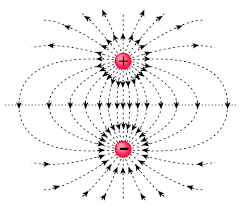
\includegraphics[width=99.75pt,height=99.75pt]{dipole-field.png}};
%Straight Lines [id:da6792737911619806] 
\draw    (517,277) -- (517,29.4) ;
\draw [shift={(517,27.4)}, rotate = 90] [fill={rgb, 255:red, 0; green, 0; blue, 0 }  ][line width=0.08]  [draw opacity=0] (12,-3) -- (0,0) -- (12,3) -- cycle    ;
%Straight Lines [id:da4136268135430723] 
\draw [color={rgb, 255:red, 74; green, 144; blue, 226 }  ,draw opacity=1 ][line width=1.5]    (517,251) -- (517,198.4) ;
\draw [shift={(517,194.4)}, rotate = 90] [fill={rgb, 255:red, 74; green, 144; blue, 226 }  ,fill opacity=1 ][line width=0.08]  [draw opacity=0] (15.6,-3.9) -- (0,0) -- (15.6,3.9) -- cycle    ;
%Straight Lines [id:da5882193234619546] 
\draw [color={rgb, 255:red, 74; green, 144; blue, 226 }  ,draw opacity=1 ][line width=1.5]    (517,127.4) -- (517,74.79) ;
\draw [shift={(517,70.79)}, rotate = 90] [fill={rgb, 255:red, 74; green, 144; blue, 226 }  ,fill opacity=1 ][line width=0.08]  [draw opacity=0] (15.6,-3.9) -- (0,0) -- (15.6,3.9) -- cycle    ;
%Straight Lines [id:da21684822857397124] 
\draw [color={rgb, 255:red, 80; green, 227; blue, 194 }  ,draw opacity=1 ][line width=1.5]    (504,122) -- (504,84.4) ;
\draw [shift={(504,80.4)}, rotate = 90] [fill={rgb, 255:red, 80; green, 227; blue, 194 }  ,fill opacity=1 ][line width=0.08]  [draw opacity=0] (15.6,-3.9) -- (0,0) -- (15.6,3.9) -- cycle    ;

%Image [id:dp5512957233213471] 
\draw (183.5,143.5) node  {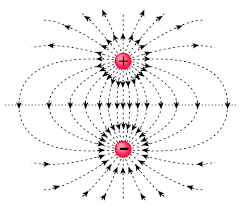
\includegraphics[width=99.75pt,height=99.75pt]{dipole-field.png}};
%Straight Lines [id:da5660597373419685] 
\draw    (67,144) -- (332,144) ;
\draw [shift={(334,144)}, rotate = 180] [fill={rgb, 255:red, 0; green, 0; blue, 0 }  ][line width=0.08]  [draw opacity=0] (12,-3) -- (0,0) -- (12,3) -- cycle    ;
%Straight Lines [id:da2620319569768228] 
\draw [color={rgb, 255:red, 74; green, 144; blue, 226 }  ,draw opacity=1 ][line width=1.5]    (185,172) -- (185,119.4) ;
\draw [shift={(185,115.4)}, rotate = 90] [fill={rgb, 255:red, 74; green, 144; blue, 226 }  ,fill opacity=1 ][line width=0.08]  [draw opacity=0] (15.6,-3.9) -- (0,0) -- (15.6,3.9) -- cycle    ;
%Straight Lines [id:da16953873290054022] 
\draw [color={rgb, 255:red, 80; green, 227; blue, 194 }  ,draw opacity=1 ][line width=1.5]    (272,160) -- (272,122.4) ;
\draw [shift={(272,164)}, rotate = 270] [fill={rgb, 255:red, 80; green, 227; blue, 194 }  ,fill opacity=1 ][line width=0.08]  [draw opacity=0] (15.6,-3.9) -- (0,0) -- (15.6,3.9) -- cycle    ;
%Straight Lines [id:da8731747530295029] 
\draw [color={rgb, 255:red, 74; green, 144; blue, 226 }  ,draw opacity=1 ][line width=1.5]    (280,172) -- (280,119.4) ;
\draw [shift={(280,115.4)}, rotate = 90] [fill={rgb, 255:red, 74; green, 144; blue, 226 }  ,fill opacity=1 ][line width=0.08]  [draw opacity=0] (15.6,-3.9) -- (0,0) -- (15.6,3.9) -- cycle    ;

% Text Node
\draw (529,20.4) node [anchor=north west][inner sep=0.75pt]    {$z\ \text{mode}$};
% Text Node
\draw (207,320) node [anchor=north west][inner sep=0.75pt]   [align=left] {(a)};
% Text Node
\draw (509,320) node [anchor=north west][inner sep=0.75pt]   [align=left] {(b)};
% Text Node
\draw (336,144) node [anchor=west] [inner sep=0.75pt]    {$x,y\ \text{modes}$};


\end{tikzpicture}
